\section{Durchführung}
\label{sec:Durchführung}

% Der verwendete Aufbau ist in \autoref{fig:aufbau} dargestellt. Er besteht aus einer Rubidiumdampflampe, um Photonen
% mit der Energie der $D_1$-Linie zu emittieren. Das Licht wird anschließen durch eine Linse gebündelt, mit Hilfe
% Interferenzfilters auf die $D_1$-Komponente reduziert und durch ein $\lambda/4$-Plättchen zirkular polarisiert.
% Danach durchquert es eine mit Rubidiumdampf gefüllte Zelle, um durch eine weiter Linse fokussiert zu werden und
% an einer Photodiode detektiert zu werden. Die Rubidium Zelle wird auf $\SI{50}{\celsius}$ geheizt, um Dampf zu
% erzeugen.
% \begin{figure}
%     \centering
%     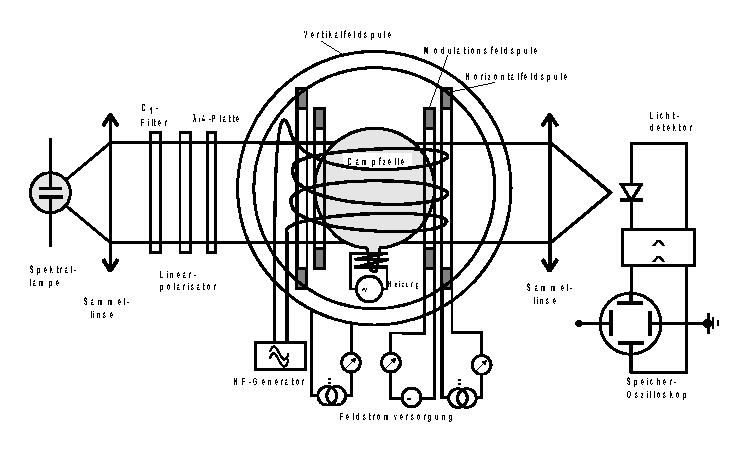
\includegraphics[scale=0.8]{pictures/Aufbau2.pdf}
%     \caption{Schematische Darstellung des verwendeten Versuchaufbaus. \cite{v21}}
%     \label{fig:aufbau}
% \end{figure}
% Die Zelle wird von drei Helmholtzspulenpaaren umgeben. Ein Vertikales, das dazu verwendet wird das Erdmagnetfeld
% auszugleichen. Die anderen beiden werden in der Horizontalen verwendet, um das RF-Feld
% zu erzeugen. Die Ausgabe der Photodiode kann an einem Oszilloskop abgelesen werden, das es im Sweep-Modus erlaubt
% verschiedene Feldstärken zu überstreichen, um eine möglichst genaue Messung zu bekommen. Der Aufbau wird nach der
% entsprechenden Justierung abgedeckt, um Umwelteinflüsse möglichst gering zu halten.


% Zu Beginn wird der Versuchsaufbau justiert und der Tisch in Richtung des Erdmagnetfelds ausgerichtet. Auf dem
% Oszilloskop ist nach Einschalten der Apparatur ein breiter Peak zu sehen, der sich auf das Abfallen der
% Transparenz bei fehlendem Magnetfeld zurück führen lässt. Durch Einstellen des Vertikalfeldes wird nun das
% Erdmagnetfeld kompensiert und dadurch der Peak schmaller gemacht. Danach werden die beiden Rubidiumisotope auf
% ihre Resonanzstellen untersucht. Dazu wird die RF-Spule eingeschaltet und Messwerte im Bereich von
% $\SI{100}{\kilo\hertz}$ bis $\SI{1}{\mega\hertz}$ in $\SI{100}{\kilo\hertz}$-Schritten aufgenommen. Für die
% höheren Frequenzen wird zusätzlich noch ein anderes horizontales Feld angelegt. Außerdem wird noch ein Bild eines
% typischen Kurvenverlaufs am Oszilloskops fotografiert.



\autoref{fig:aufbau} veranschaulicht den verwendeten Versuchsaufbau.
\begin{figure}
    \centering
    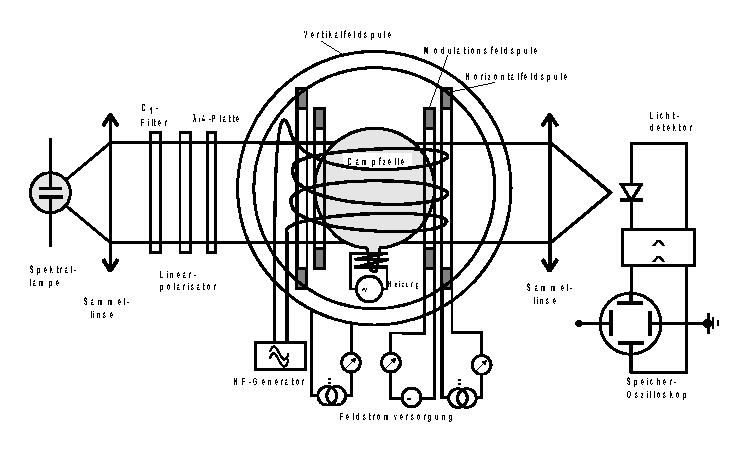
\includegraphics[width=0.95\textwidth]{pictures/Aufbau2.pdf}
    \caption{Schematische Darstellung des verwendeten Versuchaufbaus. \cite{v21}}
    \label{fig:aufbau}
\end{figure} 

Dieser besteht aus einer Rubidiumdampflampe, die Photonen mit der Energie der $D_1$-Linie emittiert. 
Das erzeugte Licht der Wellenlänge $\lambda = \qty{794.8}{nm}$ wird mithilfe einer Linse gebündelt und 
durch Interferenzfilter auf die $D_1$-Komponente reduziert. 
Anschließend wird es durch ein $\lambda/4$-Plättchen zirkular polarisiert. 
Das polarisierte Licht durchläuft eine mit Rubidiumdampf gefüllte Zelle
und wird durch eine weitere Linse fokussiert, um schließlich von einer Photodiode detektiert zu werden. 
Um Dampf zu erzeugen, wird die Rubidiumzelle etwa eine halbe Stunde vor Beginn der Messung auf eine Temperatur von $\SI{50}{\celsius}$ erhitzt.

Die Dampfzelle ist von drei Paaren von Helmholtzspulen umgeben. 
Eine vertikale Spule wird verwendet, um das Erdmagnetfeld auszugleichen, 
während die beiden horizontalen Spulen verwendet werden, um das RF-Feld zu erzeugen. 
Die Ausgabe der Photodiode kann auf einem Oszilloskop im Sweep-Modus angezeigt werden, 
wodurch verschiedene Feldstärken abgedeckt werden können, um präzise Messungen zu ermöglichen. 
Um Umwelteinflüsse zu minimieren, wird der Aufbau nach entsprechender Justierung abgedeckt.

Zu Beginn wird der Versuchsaufbau justiert und der Tisch in Ausrichtung des Erdmagnetfelds positioniert. 
Aufgrund des fehlendem Magnetfeld und der daher sinkenden Transparenz
ist nach Einschlaten der Apparatur auf dem Oszilloskop ein Peak zu erkennen.
Durch Anpassung des Vertikalfeldes wird das Erdmagnetfeld kompensiert und der Peak wird schmaler. 
Anschließend werden die beiden Rubidiumisotope auf ihre Resonanzstellen untersucht. 
Hierfür wird die RF-Spule aktiviert und Messwerte im Frequenzbereich 
von $\SI{100}{\kilo\hertz}$ bis $\SI{1}{\mega\hertz}$ in Schritten von $\SI{100}{\kilo\hertz}$ aufgezeichnet. 
Für höhere Frequenzen wird zusätzlich ein anderes horizontales Feld angelegt.